\documentclass[journal]{IEEEtran}

%\usepackage{ifpdf}
\usepackage{cite}
\usepackage{graphicx}
\usepackage[cmex10]{amsmath}
\usepackage{algorithmic}
%\usepackage{array}
\usepackage[caption=false,font=footnotesize]{subfig}
%\usepackage{fixltx2e}
%\usepackage{stfloats}
%\usepackage{dblfloatfix}
\usepackage{url}
\hyphenation{op-tical net-works semi-conduc-tor}

%% wrap algorithm in a figure environment without caption and number.
%% #1 is the title of the algorithm.
\newenvironment{myalgorithm}[1]%
{\begin{figure}[!h]\small\noindent\rule{\linewidth}{1pt}\\#1\vspace{-0.5em}\\%
\rule{\linewidth}{0.5pt}\\\vspace{-1.5em}}%
{\vspace{-0.5em}\rule{\linewidth}{1pt}\end{figure}}

\begin{document}
\title{Hypercolumn-array Based Image Representation and 
Its Application to Shape-based Object Detection}
\author{Hui~Wei\thanks{Hui~Wei is with the School of Computer Science, 
Laboratory of Cognitive Modeling and Algorithms, 
Brain Science Research Center, Fudan University, Shanghai, China. 
Corresponding author's email: weihui@fudan.edu.cn.},
Zheng~Dong\thanks{Zheng~Dong and Qiang~Li are with the School of Computer Science, 
Laboratory of Cognitive Modeling and Algorithms, 
Fudan University, Shanghai, China.},
and~Qiang~Li}

% The paper headers
%\markboth{Journal of \LaTeX\ Class Files,~Vol.~13, No.~9, September~2014}%
%{Shell \MakeLowercase{\textit{et al.}}: Bare Demo of IEEEtran.cls for Journals}
%\IEEEpubid{0000--0000/00\$00.00~\copyright~2014 IEEE}
% Remember, if you use this you must call \IEEEpubidadjcol in the second
% column for its text to clear the IEEEpubid mark.

% make the title area
\maketitle

\begin{abstract}
Machine learning is perhaps the most popular strategy currently employed in object recognition. 
The strategy typically uses a high-dimensional vector to describe an image, 
and applies some classification algorithm to isolate positive areas apart from negative areas. 
While the advantage of this strategy is its architectural simplicity, 
it simultaneously suffers from computational complexity, fragile representation, 
unguaranteed generalization, black arts in optimization, and so on. 
In comparison with low-order features, such as color or gradient, contour is more stable and persistent; 
therefore, shape-based methods take account of a greater number of essential aspects for object recognition. 
Biological and psychological evidence increasingly reveals that geometrical and topological features are the keys to object recognition. 
Although these types of high-level features are not easily obtained, 
their discriminating abilities greatly improve the efficiency of perception. 
Attracted by the excellent performance of neural visual systems for shape processing, 
we simulate the mechanism of hypercolumns in the V1 cortex of mammals that selectively responds to bar stimuli, 
and design an orderly-arranged array to extract and represent all possible linear or near-linear stimuli in an image. 
Each unit of this array can cover all orientation stimuli occurring over a certain small area. 
These effective units together produce a type of low-dimensional vector to describe shape. 
Based on the neighborhood of units in the array, 
we construct a graph whose node represents a short line segment with a certain position and slope. 
Therefore, any segment of contour, i.e., a curve, in an edge image might be a route in that graph. 
The most significant thing here is that a graph converts an image, comprised of typically unstructured raw data, 
into structured and semantic-enriched data. 
We search along the routes in that graph and compare them with a shape template for object detection. 
Organizing segments of contour into a graph greatly upgrades the level of image representation, 
remarkably reduces the load of combinations, significantly improves the efficiency of object searching, 
and facilitates the intervening of high-level knowledge. 
This work provides a systematic infrastructure for shape-based models.
\end{abstract}

% Note that keywords are not normally used for peerreview papers.
\begin{IEEEkeywords}
orientation column, shape representation, object recognition, primary visual cortex.
\end{IEEEkeywords}

\IEEEpeerreviewmaketitle

\section{Introduction}

% needed in second column of first page if using \IEEEpubid
%\IEEEpubidadjcol

\IEEEPARstart{D}{etecting} 
an object within a complex background is still one of the major challenges of pattern recognition and computer vision. 
The difficulty lies in the conditions of image capture,
where images are captured under different illumination conditions, 
from different distances, and, sometimes, with overlapping objects.
These variations make an object's appearance, either in size, in posture, or in color, endless changing. 
While machine learning is arguably the most popular strategy currently employed in object recognition, 
the uncertainties associated with an ever changing environment and limited training create numerous difficulties for machine learning methods to achieve efficient object recognition. 
As such, obtaining an efficient, stable, and convenient method of representing features becomes the key requirement of object recognition in the real-world. 
The most stable characteristic of an object is its contour. 
The shapes or contours of most rigid objects tend to remain invariant regardless of a changing environment. 
Therefore, an object's shape or contour represents the most promising feature for efficient object recognition.


The primary visual cortex, which is also known as V1, locates in the striate cortex of mammals.
It is the best-studied visual area in the brain.
In this paper, we simulate the neural mechanism of V1 because this area contains many orderly-arranged hypercolumns that represent the orientation information of a visual stimulus.
This biological infrastructure provides a feasible entity to record object contours. 
We therefore design and train a self-organizing map (SOM) to extract the line information of an image. 
Under this approach, any line, regardless of its position, length, or slope, 
will activate one or more orientation-sensitive neurons, 
so an edge-image will be re-described by a set of active neurons. 
Based on this line-representing platform, 
we propose a contour-matching algorithm that uses geometrical characteristics to recognize objects. 
This provides good performance in environment adaptation and better generalization.

The remainder of this paper has been organized as follows. 
Section 2 reviews some related studies in shape-based object recognition and visual neurobiological mechanism simulation. 
The advantages and disadvantages of the main features of each study are briefly discussed. 
Section 3 presents the training process involving orientation columns, 
and how an image is represented by an array of artificial orientation columns. 
Section 4 describes how an edge image is converted into an undirected graph, 
and how route searching is conducted for this graph. 
Section 5 presents the method of similarity matching between routes and templates, 
and how this method is applied to the recognition of objects in real images. 
Experimental results are presented in Section 6, which is divided into two parts. 
Part one analyzes the capability for image representation and reduction provided by the proposed array of artificial orientation columns. 
Part two presents the recognition results obtained for some real image datasets. 
The final section presents conclusions and future expectations.

\section{Related Work}

Here, we divide the discussion of related work into two components. 
One component concerns the modeling of the V1 area, 
whereas the other component is concerned with shape- or contour-based object recognition methods. 

\subsection{V1 simulation research}

A number of approaches to the computational modeling of the neural mechanism of the V1 area of mammals have been proposed. 
The differences between these approaches lie in their points of focus, 
where some approaches focus on pathway, some on mechanism, and some on computation. 
Some studies have concentrated on the visual neural pathway 
\cite{bickle1999,shariati2012,nakagama2004,harvey2008}. 
For example, Bickle et al. \cite{bickle1999} proposed an artificial neural network with interactive activation and competition (IAC) mechanism by reference to the lateral geniculate nucleus (LGN), 
which is the direct pathway from the primary visual cortex to the thalamus, 
to implement several functions of the visual cortex. 
Shariati et al. \cite{shariati2012} simulated the entire neural pathway from a photoreceptor in the retina to the second sub-layer of the primary visual cortex. 
Some studies have concentrated on visual neurocomputing problems 
\cite{curuklu2002,wang2011,li2005,mihalas2011,ramirez2013}. 
For example, Curuklu \cite{curuklu2002} proposed a Bayesian confidence propagation neural network (BCPNN) to simulate a hypercolumn, which is the functional unit of the visual cortex. 
Wang et al. \cite{wang2011} used sparse coding and a back-propagation (BP) neural network to model the primary visual cortex. 
Finally, a number of studies have concentrated on the functional roles of variant neurons in the visual system \cite{okamoto2004,willmore2012,bednar2012,law2011,giacomantonio2010,zhao2010,yan2012,piech2013,song2013}. 
Okamoto \cite{okamoto2004} designed a honeycomb-like model based on a mechanism of short-range horizontal connections to explain the topological characteristics of the V1 area. 
Willmore \cite{willmore2012} successfully simulated the visual cortex based on Hebbian and anti-Hebbian rules. 
Bednar et al. \cite{bednar2012,law2011} implemented a gain-controlled, adaptive, 
and lateral-connected model that specialized the function of every neuron in the pathway, 
and simulated the primary visual cortex more completely. 
The above studies were able to realize some neural circuits and partial functions of the V1 area.
However, they did not sufficiently account for real image representation, 
which is the ultimate and most important function of the V1 area. 
In fact, all subsequent processing, such as object recognition and scene understanding, 
begins in the V1 area. 
Above all, these studies lacked the crucial consideration of how the V1's output meets the demands of subsequent recognition tasks. 
This constitutes one of the main goals of the present study.

\subsection{Shape- or contour-based object recognition}

Shape- or contour-based object recognition research has a long history. 
In the early stage, chamfer matching \cite{borgefors1988,shotton2005,thayananthan2003,opelt2006} 
was a frequently-used method that converted an original image into a depth image, 
and searched for the point with the best match. 
This method demonstrated a certain adaptability. 
As an additional aid, an image pyramid was designed to achieve scale invariance \cite{borgefors1988}. 
However, this method usually exhibits high time complexity and has a low tolerance to background interference. 
To address this problem, several new variants of the chamfer matching method have been proposed in recent years. 
For example, Shotton \cite{shotton2005} designed an oriented chamfer matching model, 
Thayananthan \cite{thayananthan2003} combined this method with a shape context descriptor, 
and Opelt \cite{thayananthan2003} added AdaBoost. 
These variants were observed to improve the efficiency and recognition rate.

Another type of shape-based method is mainly based on contour segment matching between templates and real images. 
This type of method firstly converts an image into edges, 
and then fits curves or line segments to the edge pixels. 
Subsequently, the set of curves or line segments are represented with some geometrical feature descriptors. Finally, the similarity between the set of segments and shape templates are obtained. 
Once matching pairs between line segments and the template are established, 
some guesses can be made to estimate the possible positions for the target object, 
and then verify these possible positions one-by-one. 
This type of method can be further divided into two categories. 
One is the dominant-set method and the other is the partial-match method. 
Pavan \cite{pavan2007} proposed the dominant-set method for finding the principle corresponding components in two sets. 
Yang \cite{yang2012} used this method to form a scale invariant global shape similarity estimation to match between template contour parts and image edge fragments. 
Partial-match methods \cite{ma2011,riemenschneider2010,liu2010} are similar to dominant-set methods. 
Ma \cite{ma2011} obtained a similarity matrix based on the angles of edges in a contour and maximized the similarity between classes through Liu's cluster algorithm \cite{liu2010}. 
Objects were then recognized by seeking the largest community. 
Differing from the work of Ma \cite{ma2011}, 
in the stage of evaluation, Riemenschneider \cite{riemenschneider2010} estimated the object position using the pyramid matching kernel (PMK) algorithm after conducting contour segment matching. 
Methods proposed in \cite{zhu2008,srinivasan2010} introduced a shape context descriptor. 
Zhu \cite{zhu2008} used linear programming to find a one-to-one mapping between the image and the template. 
Srinivasan \cite{srinivasan2010} developed this method further by introducing a bottom-up process to optimize many-to-one mapping results. 
In general all these methods exhibit high time complexity subject to exhaustive comparison between real-world images and templates.

Other shape-based recognition methods have been proposed, 
such as the constellation model \cite{fergus2004} and spectral model \cite{leordeanu2007}.
These methods use the relative location of points in a contour, 
where the established spatial relationships are regarded as constraints. 
The spatial relationships of an edge point to its surroundings are calculated in order to 
determine whether the surrounding pixels belong to the target object or to the background. 
A sparse representation is thus derived from these spatial relationships, 
and a probabilistic inference is used to estimate the position of a target object. 
The main disadvantage of this type of method is that the recognition result can be greatly affected 
when the foreground and the background are mixed or objects overlap. 
Leordeanu \cite{leordeanu2007} proposed a spectral model to calculate the geometrical relationships of pairwise points, 
and to analyze where pairwise points were densely located in a contour. 
The drawback of this model is that it requires a great many training samples.

In addition, some shape-based recognition methods are a mixture of several existing approaches. 
Fergus \cite{fergus2004} counted the occurrences of foreground features, 
and consulted with contour matching to obtain the probabilities of foreground to background, 
and, finally, to estimate the position of a target object. 
Gupta \cite{gupta2009} designed a contour descriptor by reference to the concept of torsion in physics. 
This descriptor performs well for changing scales. 
However, the method performs poorly when the contour is somewhat missing because it is concerned with global contours. 
Schlecht \cite{schlecht2011} described the marked features of an object by a codebook of angles, 
and combined Hough voting for object detection. 
Ferrari \cite{ferrari2006} proposed gradual contour searching to recognize objects in a real-world image.

In general, shape-based object recognition methods are not covered by the mainstream technology. 
The reasons for this are as follows. 
(a) This type of method always requires good preprocessing to reduce noise or to obtain some basic geometrical units such as line segments; however the preprocessing results are affected by numerous factors. 
(b) A target object’s background, position, size, and posture are changing constantly, 
which is a substantial challenge for template matching. 
(c) Template matching is essentially a combinational optimization problem that requires searching for a globally optimum solution, 
which is a severe challenge for any searching algorithm. 
(d) The template matching method involves many process steps such as template acquisition, 
template formal representation, search-friendly image re-organization and re-representation after preprocessing, 
definition of geometrical features, searching and combining geometrical features, 
definition of geometrical constraints, and generating and verifying assumptions. 
All these requirements increase the complexity of a complete shape-based system.

\section{Hypercolumn-array Based Image Representation}

\subsection{The structure of a hypercolumn-inspired array}

In \cite{wei2014,wei2014b,wei2000}, 
a multi-layer neural computational model that simulated hypercolumns in the primary visual cortex was proposed. 
The output layer of this model can be used to represent the orientation information of a contour image.

\begin{figure}[!t]
\centering
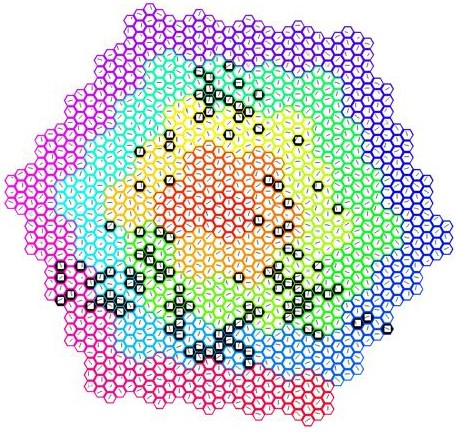
\includegraphics[width=0.85\linewidth]{images/fig1.jpg}
\caption{The structure of a hypercolumn-array, which is used for contour representation. 
Each small hexagon represents an orientation chip that corresponds to a simple cell. 
Each simple cell in the V1 area is sensitive to a bar of light with a particular orientation (slope). 
We evenly divide the overall orientation interval from 0 to $\pi$ into nineteen sub-intervals. 
Nineteen orientation chips, each of which responds to one, and only one, sub-interval, 
are combined as a hypercolumn, and nineteen small hexagons happen to form a large hexagon. 
All the chips in the same hypercolumn share the same receptive field.}
\label{fig:1}
\end{figure}

As shown in \figurename~\ref{fig:1},
this layer is comprised of a number of large, hexagonal hypercolumns, 
and two of these in the upper-right corner of the figure are marked by two black frames. 
Each hypercolumn consists of nineteen orientation chips (small hexagons). 
Each chip can selectively respond to an orientation-specific segment of contour existing in its receptive field. 
\figurename~\ref{fig:2} shows the scope and the distribution of the receptive fields of several neighboring hypercolumns, and how they share these receptive fields. 
All nineteen chips in a single column can completely cover the range of slope from 0 to $\pi$. 
All these columns assemble into an array, 
which plays the roles of extraction and representation of the orientation features of contour in an image. 

\begin{figure}[!t]
\centering
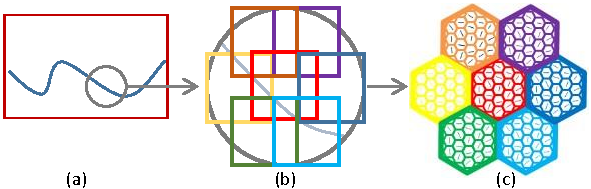
\includegraphics[width=\linewidth]{images/fig2.pdf}
\caption{Seven neighboring hypercolumns and their receptive fields in a visual field. 
(a) A segment of contour in a visual field. 
(b) The purple rounded region is covered by seven square receptive fields, 
and they overlap with each other to some extent. 
(c) Seven colored neighboring hypercolumns whose corresponding receptive fields with the same colors 
are shown in (b).}
\label{fig:2}
\end{figure}

\subsection{Representing images by a hypercolumn-inspired array}

One of the most important discoveries in neurobiology is that a hypercolumn in the primary cortex can respond to a series of stimuli with continuously changing orientations. 
As the discoverers, Hubel and Wiesel won the Nobel Prize in 1982. 
We were therefore inspired to use this mechanism to obtain and represent segments of contour in an image. 
After uploading an edge image to the aforementioned hypercolumn array, 
in a certain receptive field, 
some linearly-distributed pixels will activate a certain orientation chip of a hypercolumn. 
This indicates that we can represent all contour information in an image by a set of active units (i.e., orientation chips). In mathematics, each unit represents a line vector. Therefore, the output of a hypercolumn array is no longer a group of discrete, isolated, and pixel-wise points, 
but some preliminarily-integrated short line segments that contain a wealth of geometrical information such as position, length, and angle. 
Thus, the hypercolumn array not only upgrades the representation level of an edge image, 
but also reserves the original characteristic of pixel distribution in an edge image. 
\figurename~\ref{fig:3} to \figurename~\ref{fig:5} shows several examples of such representation.
A simple triangle, an onion shape, and a contour of a car were uploaded to the hypercolumn array,
which generated a set of activated orientation chips.
This is very similar to using sparse coding to represent an image.

\begin{figure}[!t]
\centering
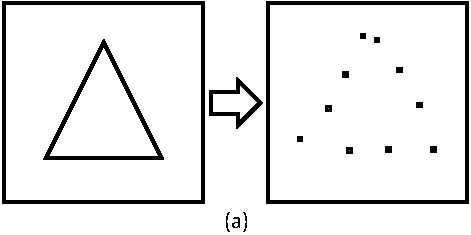
\includegraphics[width=0.55\linewidth]{images/fig3.pdf}
\caption{Some orientation chips (black points in (b)) are activated by a simple triangle in (a), 
where, in (b), the topological feature of the triangle is preserved by the set of active orientation chips.}
\label{fig:3}
\end{figure}

\begin{figure}[!t]
\centering
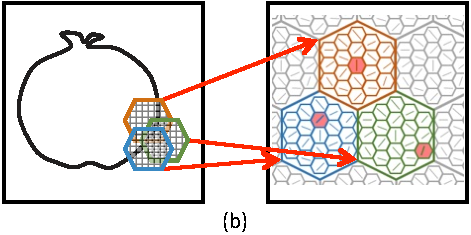
\includegraphics[width=0.55\linewidth]{images/fig4.pdf}
\caption{The partial contour at the bottom-right of an onion (in (a)) from the MPEG7 dataset 
passes through three neighboring and overlapping receptive fields, 
which activates three orientation chips in the three hypercolumns respectively (in (b)), 
and these chips correctly reflect the geometrical information in this contour segment.}
\label{fig:4}
\end{figure}

\begin{figure}[!t]
\centering
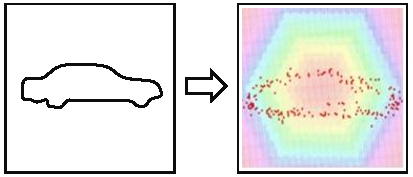
\includegraphics[width=0.55\linewidth]{images/fig5.pdf}
\caption{A contour of a car is represented by an array with 452 hypercolumns. 
The extent to which the details of the car that are preserved increases 
with an increasing number of activated orientation chips.}
\label{fig:5}
\end{figure}

The foregoing examples indicate that an edge image can be easily represented with activated orientation chips in a hypercolumn array. 
Each activated chip represents a vector reflecting the position, length, and angle of a short line segment. 
In addition, the chip's activation level can also indicate the level of similarity between a real stimulus and the chip's built-in preference. 
This is equivalent to a comparison between an input and a template. 
For example, the stimulus in a receptive field might sometimes be a curve or a dotted line rather than a perfect straight line. 
Therefore, the output of hypercolumns is an approximation to the original edge image, 
as shown in \figurename~\ref{fig:6}. 
This approximation can reflect the distribution of pixels in a receptive field, which offers a certain degree of flexibility and error tolerance.

\begin{figure}[!t]
\centering
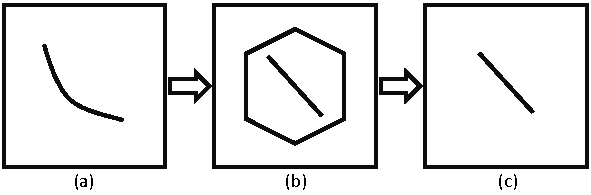
\includegraphics[width=0.6\linewidth]{images/fig6.pdf}
\caption{Orientation chips can approximately represent stimulus. 
(a) A real stimulus in a receptive field might be a small curve. 
(b) An orientation chip with the closest built-in orientation preference is activated. 
(c) The final output is an approximation of the original stimulus.}
\label{fig:6}
\end{figure}

\subsection{Image reconstruction from an activated array}

However, the scale of a hypercolumn-array, given as the number of hypercolumns in it, 
and the number of orientation chips in a hypercolumn, is limited. 
Thus, using a finite resource to represent infinite stimuli must inevitably result in approximation, 
and the degree of approximation must be evaluated after converting an original image to some activated orientation chips. 
To verify that the hypercolumn array can represent the original stimulus with sufficient fidelity, 
we rebuild an image by redrawing lines in the receptive fields of the activated orientation chips, 
and then compare the original image to the rebuilt one. 
As shown in \figurename~\ref{fig:7}, 
the contour information of an original image can be effectively recorded, 
and the rebuilt version is nearly identical to the original. 
Further experimental verification of the image reconstruction ability of a hypercolumn-array will be presented in Section 6.

\begin{figure}[!t]
\centering
\subfloat[Original image]{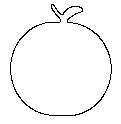
\includegraphics[width=0.25\linewidth]{images/fig7a.jpg}%
\label{fig:7a}}
\hfil
\subfloat[Rebuilt image]{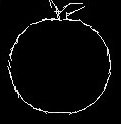
\includegraphics[width=0.25\linewidth]{images/fig7b.jpg}%
\label{fig:7b}}
\caption{The result of image reconstruction. (a) An original image from the MPEG7 dataset. (b) A rebuilt image based on the orientation chips activated by (a). Here, (a) and (b) are nearly identical.}
\label{fig:7}
\end{figure}

\section{Processing From A Hypercolumn Array To A Graph}

After the preprocessing of the hypercolumn array discussed in the previous section, 
an ordinary edge image has been converted to a group of active units, 
each of which represents a short line segment with a certain position, length, and slope, 
given as a quad vector: $x$-coordinate of the center point, 
$y$-coordinate of the center point, length, and slope. 
This representation by a group of units is more compact and information-rich. 
Compared with a complete contour, the line segment represented by an active unit is somewhat fine, 
and the information obtained from active units must be aggregated in some way to facilitate the subsequent recognition operation. 
The use of sets is a simple aggregation approach, 
but this approach is not sufficiently powerful to describe the topology of active units distributed in an array. 
The use of graphs is a more effective approach to describe the relations between adjacent or connected active units. 
Moreover, the layout characteristics of chips arranged in a hypercolumn as well as hypercolumns arranged in an array coincide with the functionality of graphs, 
where nodes and edges are two basic elements for constructing a graph. 
The analogy between a hypercolumn-array and a graph is quite a natural association. 
This suggests the application of graphs to describe the topological distribution of activated orientation chips.

\subsection{The generation of a graph}

We hope to represent a continuous contour by coordinating the information derived from multiple chips through the implementation of a graph. 
Therefore, the best manner of defining a graph for a hypercolumn-array is to set the chips as the nodes of the graph, 
and establish the edges between those nodes (i.e., chips) that might be successively joined together to represent a slightly longer line or curve. 
Because all 19 chips in a given hypercolumn share a completely coincident receptive field, 
and multiple lines are unlikely to exist concurrently in this fairly small area, 
these chips are usually not activated simultaneously.
Therefore, no edges can be established between these independent nodes. 
Only those chips with neighboring or partially overlapping receptive fields might be coordinated to represent a contour that passes through multiple receptive fields. 
Links are assigned between these possibly coordinated nodes that usually belong to separate but adjacent hypercolumns. 
The present description defines a basic graph of chip nodes, i.e., an orientation chip graph. 
Once an image has been uploaded, 
some nodes of this graph will be activated. 
Most importantly, the orientation chip graph provides a structural data form for subsequent geometrical or topological analysis, as illustrated in \figurename~\ref{fig:8}.

\begin{figure}[!t]
\centering
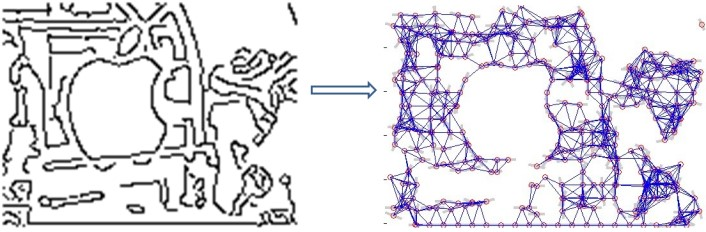
\includegraphics[width=0.85\linewidth]{images/fig8.jpg}
\caption{An edge image from the ETHZ dataset (at left) has activated some orientation chips. 
We can generate an undirected graph (at right), of which the nodes are these activated chips.}
\label{fig:8}
\end{figure}

\subsection{Graph searching and route-parsing}

The most significant value provided by the graph of chip nodes is 
(a) it effectively organizes raw image data, which is converted into an ordered structure, 
and (b) it facilitates the process of searching object contours. 
As indicated by the previous discussion, 
representing a continuous contour requires the coordination of multiple chips, 
which correspond to multiple connected nodes in our graph.
From the point of view of a graph, the sequence of these connected nodes forms a route.
\figurename~\ref{fig:9} shows an example of a route. 
The key to shape-based object recognition involves locating one or several such routes
that represent the contour or partial contour of the object to be discriminated.
Therefore, a route-searching algorithm is required.

\begin{figure}[!t]
\centering
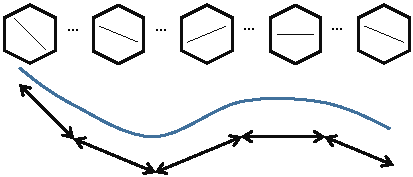
\includegraphics[width=0.5\linewidth]{images/fig9.pdf}
\caption{A segment of an object's contour might be a route of a chip graph. 
The top is a sequence of chips linked together by a route; 
the middle is the original stimulus that activated the above route; 
and the bottom is the approximate curve rebuilt from that route. }
\label{fig:9}
\end{figure}

Route-searching seeks to combine the neighboring nodes of a graph into routes that represent contour segments. 
However, some difficulties are encountered in this process because the contour of an object might suffer from interference with its background and be mixed with noise or be broken into several shorter segments.
As is shown in \figurename~\ref{fig:8}, 
the connectivity of a graph constructed from activated orientation chips can be high.
A randomly chosen long route might go through both an object and its background.
Ideally, a route should be either part of the object's contour or from the background,
and also it should convey enough information for us to determine whether it is part of the object's contour.
Therefore the searching process must be carefully guided to yield a reasonable result.
Natural contours tend to be smooth and continuous, which provides a good hint.
We assign weights to edges to measure the smoothness and continuity between chip nodes.
Given two adjacent nodes $u$ and $v$ in the chip graph,
the weight $w$ of the edge $(u,v)$ is defined as follows.
\begin{equation}
w(u,v) = e^{-\max\{dist(l(u), l(v)),\lambda\cdot|\alpha(u)-\alpha(v)|\}}.
\end{equation}
In this equation, $l(\cdot)$ is the short line segment represented by the corresponding orientation chip
and $\alpha(\cdot)$ is the orientation of that chip.
The function $dist(\cdot,\cdot)$ calculates the minimal distance between the endpoints of two line segments.
It measures the continuity between the two chips.
The difference of orientation is multiplied by a factor $\lambda$ to measure the smoothness.
In this paper, the orientation is measured in degree and $\lambda$ takes $0.15$.
The edge weights range from $0$ to $1$.
Larger weights indicate stronger collinearity between chip nodes.
\figurename~\ref{fig:10} illustrates weight setting in different cases.

\begin{figure}[!t]
\centering
\subfloat[$w=e^{-\max\{0,0\}}=1$]{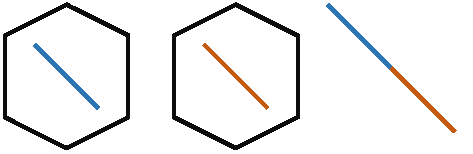
\includegraphics[width=0.45\linewidth]{images/fig10a.pdf}%
\label{fig:10a}}
\hfil
\subfloat[$w=e^{-\max\{0,15\lambda\}}=0.11$]{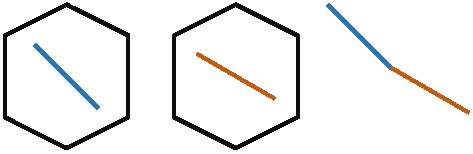
\includegraphics[width=0.45\linewidth]{images/fig10b.pdf}%
\label{fig:10b}}\\
\subfloat[$w=e^{-\max\{3,0\}}=0.05$]{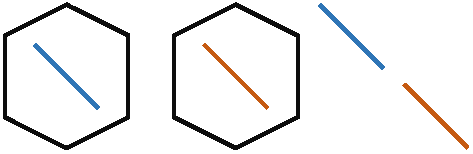
\includegraphics[width=0.45\linewidth]{images/fig10c.pdf}%
\label{fig:10c}}
\hfil
\subfloat[$w=e^{-\max\{0,35\lambda\}}=0.01$]{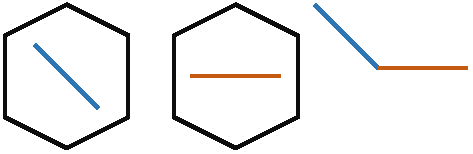
\includegraphics[width=0.45\linewidth]{images/fig10d.pdf}%
\label{fig:10d}}
\caption{Setting the edge weight between two orientation chips. 
A larger value indicates a tighter or more collinear connection.
(a) If two chips represent a longer line cooperatively, then the weight between them equals 1.
(b) If two chips represent a smooth curve, then the weight is relatively large.
(c) If two chips represent discontinuous short line segments, then the weight is small.
¨K: If two chips represent a sharp turn, then the weight is small.}
\label{fig:10}
\end{figure}

In the following Algorithm 4.1, the route searching process is guided by edge weights.
A threshold $\varpi$ for edge weight is used to control the collinearity of the routes.
In this paper, $\varpi$ takes $0.04$.
This threshold ensures that the distance between line segments represented by adjacent chips in a route are within 3 pixels and the orientation difference is less than $20^\circ$.

\begin{myalgorithm}{Algorithm 4.1 Route-Generation($G,\varpi$)}
\begin{algorithmic}[1]
\REQUIRE $G(V,E)$ is an orientation chip graph, where $V$ is the node set and $E$ is the edge set.
$\varpi$ is a threshold controlling the collinearity of routes.
\ENSURE $R$ is a set of routes found by this algorithm.
\FOR{$v\in V$}
  \STATE let $r$ be an empty route
  \WHILE{$v\neq$ nil and $v$ is not visited}
    \STATE append chip $v$ to route $r$, and mark $v$ visited
    \STATE let $\hat{u}\leftarrow$ nil
    \FOR{$u\in\{u|(u,v)\in E\textrm{ and }w(u,v)\ge\varpi\}$}
      \STATE \textbf{if} $\hat{u}$ is nil or $w(u,v)<w(\hat{u},v)$ \textbf{then} let $\hat{u}\leftarrow u$
    \ENDFOR
    \STATE let $v\leftarrow\hat{u}$
  \ENDWHILE
  \STATE \textbf{if} $r$ is not empty \textbf{then} add $r$ to $R$
\ENDFOR
\end{algorithmic}
\end{myalgorithm}

Algorithm 4.1 roughly provides some basic routes out of a graph that can be rebuilt to obtain some continuous and smooth segments of contour. 
However, there are some additional opportunities for those short basic routes to join together because 
the searching process may start from the middle of a longer route, which is broken into two segments. 
Here, we use Algorithm 4.2 to link these broken routes.

\begin{myalgorithm}{Algorithm 4.2 Route-Fusion($R,\varpi$)}
\begin{algorithmic}[1]
\REQUIRE $R$ is a set of basic routes.
$\varpi$ is a threshold controlling the collinearity of routes.
\ENSURE $R$ is updated so that short routes are joined together.
\FOR{$r_1,r_2\in R$}
  \FOR{each end node $v$ of $r_1$ and $u$ of $r_2$}
    \IF{$w(u,v)\le\varpi$}
      \STATE remove $r_1,r_2$ from $R$
      \STATE join $r_1,r_2$, and add joined route to $R$
    \ENDIF
  \ENDFOR
\ENDFOR
\end{algorithmic}
\end{myalgorithm}

Because the number of basic routes is much less than the number of nodes, 
Algorithm 4.2 usually requires less time than Algorithm 4.1. 
After the fusion process, some longer routes are obtained. 
\figurename~\ref{fig:11} presents an example. 
From this example, we can understand that the process of long-route formation can provide further integration of the edge information of an image. 
These long routes are usually lines or smooth curves. 
These routes have geometrical significance because they are no longer discrete pixels, 
and may include all or a part of the contour of an object. 
Therefore, object recognition can be realized by matching long routes with a template. 
In this phase of the process, the number of long routes is greatly reduced.
The succeeding object recognition process is thus an operation involving a small set of curves,
which is inevitably more efficient than an operation involving a large set of pixels.
  
\begin{figure}[!t]
\centering
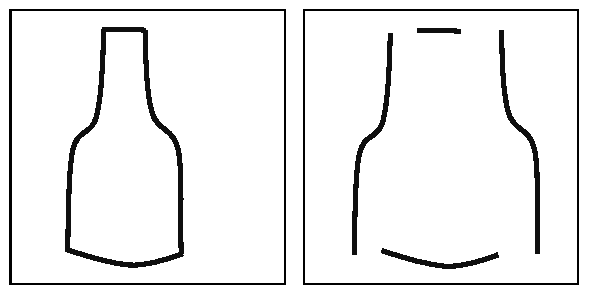
\includegraphics[width=0.45\linewidth]{images/fig11.pdf}
\caption{After conducting Algorithms 4.1 and 4.2, 
the contour of an object (at left) can be denoted by several routes (at right).}
\label{fig:11}
\end{figure}

\section{Route-based Shape Matching}

With the algorithms described in the previous section,
a set of routes are extracted from the orientation chip graph.
These routes consist of sequence of orientation chips representing continuous and smooth contour segments.
We can evaluate the similarity between these routes and the shape template. 
If a sub-graph contains many routes of high similarity to the shape template,
then it is highly possible that an object of that shape is located in the corresponding sub-region of the image which the graph represents. 
Object detection based on this idea requires two steps: 
the comparison of the similarity between a route and a segment of the template, 
and the assessment of the overall similarity between a sub-graph and the whole template.

\subsection{Measurement of similarity between a route and a template segment}

A number of algorithms exist at present for conducting curve similarity comparison. 
In \cite{schindler2008}, a curve representation method has been proposed based on a sequence of tangent angles,
but this method is not appropriate for measuring similarity between a partial contour segment and a complete shape template.
In \cite{arkin1991}, a type of turning function has been proposed to represent polygons and to measure their shapes, 
but this method is very sensitive to small zigzag or burr noise.
It is not suitable for incomplete contours or contours mixed with the background. 

Intuitively, the most direct method of comparing two curves is to evaluate the degree to which they are mutually overlapping, 
which is similar to solving an optimization problem, i.e., 
finding the best-matched interval for two curves. 
This is perhaps the most thorough method because it matches curves based upon their overall geometrical tendencies rather than local numerical features. 
Furthermore, this method can flexibly adapt to curve variances of length, position, and posture. 
We therefore designed a curve similarity measurement algorithm based on evaluating the degree of overlap between two curves. 

Here, we are concerned with two classes of curves. 
The first class, denoted as TempClass, derives from the shape template of an object category. 
The second class of curve, denoted as RouteClass, derives from routes. 
Our task is to determine whether any RouteClass curve coincides with a TempClass curve. 
The degree of coincidence represents their similarity. 
A partial match should be allowed because a RouteClass curve might include not only an object contour, 
but also a noise curve in the background. 
Therefore, the interval that maximizes the similarity is the object of optimization. 
Furthermore, rotation and scale transformations are other factors that can alter an object's contour. 
All these factors therefore make the process of seeking the best match between a template curve and a route curve an optimization process. 
\figurename~\ref{fig:12} illustrates our idea, and the algorithm is given as follows.
Algorithm 5.1 finds the optimized interval of partial match between two curves.
It is a genetic algorithm that minimizes the dissimilarity (or distance) 
between part of the RouteClass curve and the TempClass curve.

\begin{figure}[!t]
\centering
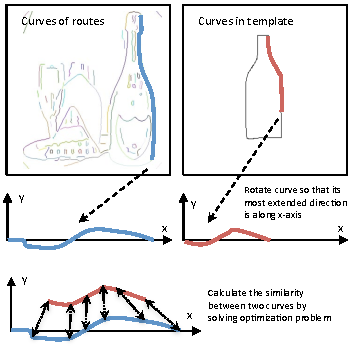
\includegraphics[width=0.8\linewidth]{images/fig12.pdf}
\caption{An example of a similarity measurement of two curves.}
\label{fig:12}
\end{figure}

\begin{myalgorithm}{Algorithm 5.1 Route-Distance($r,t$)}
\begin{algorithmic}[1]
\REQUIRE $r$ is RouteClass curve and $t$ is TempClass curve.
\STATE rotate $r$ and $t$ so that their most extended direction is along the $x$-axis
\STATE sample $t$ uniformly to $N$ points $P_t=\{(x_i,y_i)|i=1,\cdots,N\}$
\STATE randomly initialize $M$ subintervals of $[0,length(r)]$
\REPEAT
  \FOR{each subinterval $[p,q]$}
    \STATE sample $r$ in $[p,q]$ to $N$ points $P_r=\{(x'_i,y'_i)\}$
    \STATE calculate dissimilarity $d(P_t,P_r)$ by solving least-squares
  \ENDFOR
  \STATE remove 2 subintervals with maximal dissimilarity
  \STATE add 2 subintervals by shrinking and extending the one with minimal dissimilarity
\UNTIL{the minimal dissimilarity is steady}
\RETURN the minimal dissimilarity
\end{algorithmic}
\end{myalgorithm}

At the beginning of this algorithm, we rotate a curve and make its most extended direction coincide with the positive $x$-axis. 
The purpose of this step is to accommodate the posture diversity of curves. 
Interpolation is used to adjust the scale of a curve, to accommodate the scale diversity of curves. 
The dissimilarity measure $d$ is calculated by solving a least-squares problem between two point sequences,
\begin{equation}
d(P_t,P_r)=\min_{\Delta x,\Delta y,k}\sum_{i=1}^{N}(kx_i+\Delta x-x'_i)^2+(ky_i+\Delta y-y'_i)^2,
\end{equation}
where $P_t,P_r$ is the sequences of sampling points on the template curve and route curve respectively.
\figurename~\ref{fig:13} presents an example of a similarity comparison between two curves,
in which $A$ is a template, $B$ is a curve with small zigzag noise, and $C$ is a smooth curve. 
A subjective evaluation of the figure indicates that $B$ and $A$ are more alike than $C$ and $A$. 
Although $B$ has noise, its overall shape is more similar to $A$. 
The output of the similarity comparison algorithm exactly reflects this observation. 
The basic principle underlying our algorithm is that the holistic tendency in a curve is more significant for similarity measurements. 

\begin{figure}[!t]
\centering
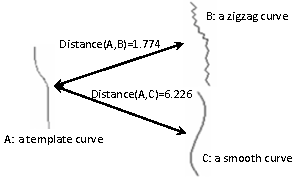
\includegraphics[width=0.65\linewidth]{images/fig13.pdf}
\caption{An example of a curve comparison based on a holistic strategy.}
\label{fig:13}
\end{figure}

\subsection{Evidence accumulation}

Based on the similarity measurement method described in the previous sub-section, 
we can enumerate the long routes determined from the chip graph one by one. 
In most cases, they will contain some discriminative segment of an object contour, 
and we can compare them with a template and label them according to their similarity values. 
This is right an evidence collecting process, 
if we see object recognition as an inference process. 
If more than a single evidence assembling at some local area of an image is observed, 
then we have reason to believe that this area deserves further searching.

A graph generated as discussed in sub-section 4.1, 
describes neighborhood relations between short line segments, 
but the number of nodes in this graph is usually great. 
According to sub-section 4.2, a graph can be decomposed into some routes, each of which represents a curve. 
This middle-level integration can greatly improve the compactness of image representation, 
and, simultaneously, create a smaller searching space. 
For instance, as shown in \figurename~\ref{fig:14}, based on 40 apple images in the ETHZ dataset, 
we respectively count the number of pixels in their edge images, the number of short line segments after hypercolumn array representation, and the number of routes after graph decomposition. 
We can see that the degree of image compactness is steadily improved, and the searching space defined by routes has been greatly reduced.

\begin{figure}[!t]
\centering
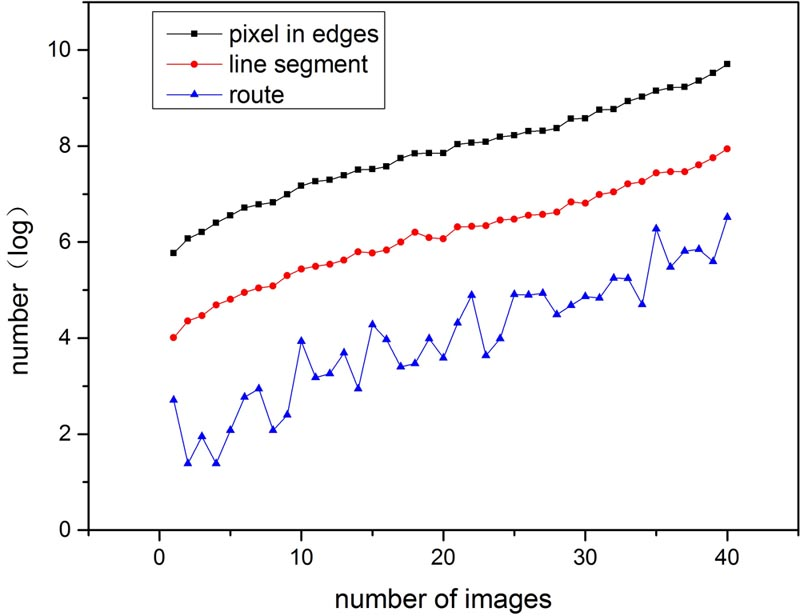
\includegraphics[width=0.7\linewidth]{images/fig14.jpg}
\caption{The Route-graph significantly reduces the searching space.}
\label{fig:14}
\end{figure}

If we assign a route as a node, and assign the neighborhood between the ends of two routes as a link, 
then we can generate a new type of graph with its grain-size enlarged. 
If the hypercolumn array based graph is denoted as a Line-graph, then this new graph is denoted as a Route-graph. 
For all nodes in the Route-graph, we define a distance matrix to measure the similarity between any pair of route curves and template curves. 
\figurename~\ref{fig:15} illustrates the formation process of this matrix. 
From each row, we can choose one or several routes with small values as evidence by which the hypothesis of a template curve occurring is supported. 
If the assemblage of evidence, i.e., those matched routes, distributes in a sufficiently narrow area, 
or if the routes are well-joined, then a goal object can be expected to occur in this area.

\begin{figure}[!t]
\centering
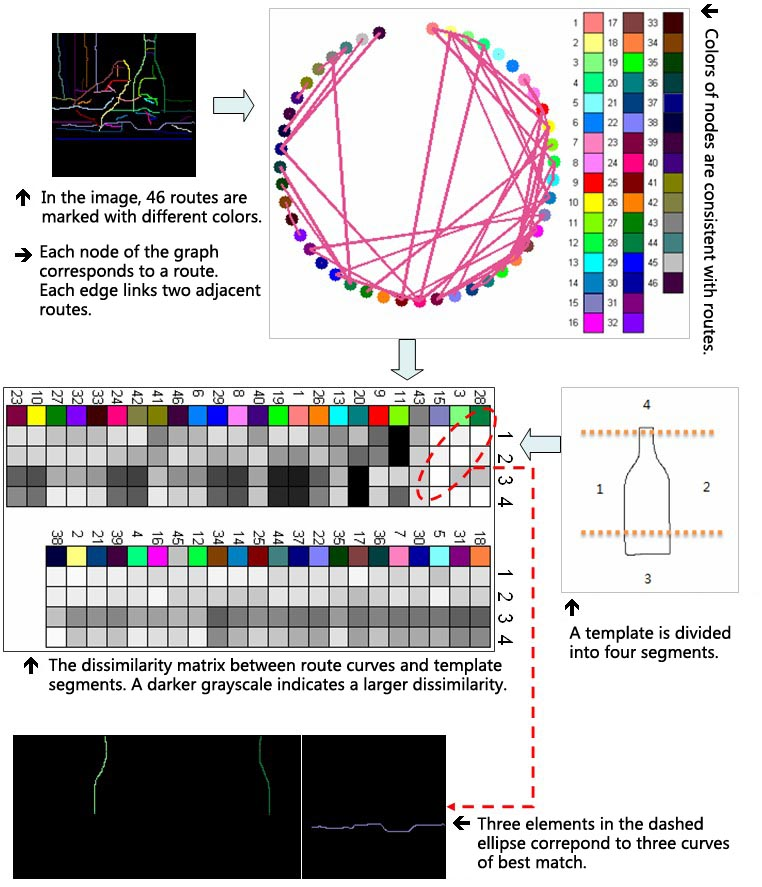
\includegraphics[width=0.98\linewidth]{images/fig15.jpg}
\caption{The distribution of evidence features among a Route-graph.}
\label{fig:15}
\end{figure}

A single factor of evidence is not sufficient for sound discrimination because this matched curve might be a part of the background. 
The co-relationships of a group of curves are more important than any single curve's similarity. 
For example, several curves that are very similar to some segments of an object's contour may be scattered over an image, but their relative spatial relations might not satisfy the structural constrains of that object. 
In this paper, we adopt two sets of independent contour partition strategies for the same template. This guarantees that the contour segments can overlap with each other to some extent. The advantage of ensuring some measure of overlap is that the joining of two adjacent segments in one set can be established by a continuous segment in another set.
We can use one set for template matching, and the other set for cross validation. 
\figurename~\ref{fig:16} illustrates this idea.

\begin{figure}[!t]
\centering
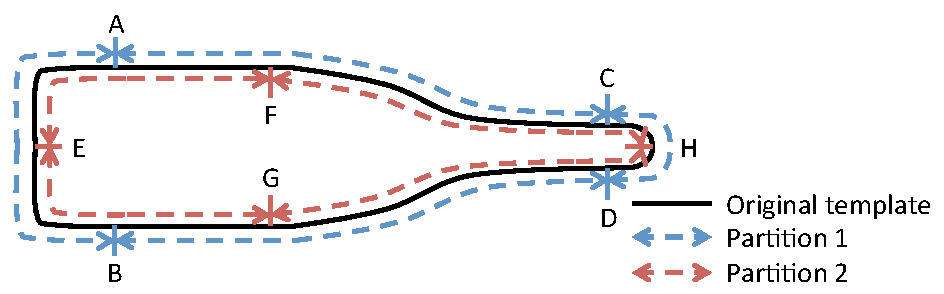
\includegraphics[width=0.8\linewidth]{images/fig16.pdf}
\caption{Two independent template partitions provide cross-verification.}
\label{fig:16}
\end{figure}

Based on the Route-graph, the following Algorithm 5.2 realizes a searching-companied matching. 
Its basic flow is as follows. 
(a) Based on the similarity between a route and template, 
a sub-graph that contains dense evidence features is detected, 
which corresponds to a likely occurrence of a goal object. 
(b) This sub-graph's route is joined with its neighboring route, 
and, if this new route exhibits an improved similarity with the template, 
then the sub-graph is updated by including the neighboring route. 
(c) A leaf node is deleted from a route, 
and, if this improves the similarity with the template, 
then the sub-graph is updated by deleting that node. 
(d) If any two neighboring routes in the sub-graph have two corresponding curves in the template, 
validate whether these two segments are adjacent or not. 
If this topological constraint of connectivity is violated, 
then update the sub-graph by deleting the shorter route. 
(e) Carry out cross-validation by altering another set of contour partition strategy.

\begin{myalgorithm}{Algorithm 5.2 Route-Graph-Object-Detection($R,T$)}
\begin{algorithmic}[1]
\REQUIRE $R$ is a set of routes. $T$ is a set of $P$ template partitions
$\{T_1,\cdots,T_P\}$. Each partition is a set of template segments.
\ENSURE the algorithm finds a subset of $R$, which corresponds to the object to be detected.
\STATE initialize a graph $G_R$ whose nodes are routes in $R$
\FOR {each $(r_1,r_2)\in R$} 
  \STATE \textbf{if} $r_1,r_2$ are adjacent \textbf{then} add edge $(r_1,r_2)$ to $E_R$
\ENDFOR
\FOR {each $T_p\in T$}
  \FOR {each $r\in R$ and $t\in T_p$}
    \STATE let $D[r][t]\leftarrow\text{Route-Distance}(r,t)$
  \ENDFOR
  \FOR {each $r\in R$}
    \STATE let $D[r]\leftarrow\min_t D[r][t]$
    \STATE let $t[r]\leftarrow\arg\min_t D[r][t]$
  \ENDFOR
  \FOR {each $t\in T_p$}
    \STATE initialize a subgraph of mere node $(\arg\min_r D[r][t])$
  \ENDFOR
  \REPEAT
    \FOR {each subgraph $G_S$}
      \STATE let $R_{adj}$ be the set of adjacent routes
      \IF {$R_{adj}\neq\emptyset$}
        \STATE add $(\arg\min_{r\in R_{adj}}D[r])$ to $G_S$
      \ENDIF
      \IF {exists $r_1,r_2\in G_S$ and $t[r_1]=t[r_2]$}
        \STATE remove the shorter of $r_1$ and $r_2$ from $G_S$
      \ENDIF
      \IF {routes in $G_S$ are more than segments in $T_p$}
        \STATE remove $(\arg\max_{r\in G_S}D[r])$ from $G_S$
      \ENDIF
    \ENDFOR
    \STATE remove duplicated subgraph
  \UNTIL {subgraphs do not change}
\ENDFOR
\RETURN the subgraph with minimal average distance
\end{algorithmic}
\end{myalgorithm}

\section{Evolution Of A Two-dimensional Template}

In previous sections, we addressed the method of object recognition using a shape template. 
However, the posture of an object is continuously changing in a natural environment, 
and all possible object postures cannot be matched to a unique template. 
This reveals a problem regarding multiple prototypes. 
The key limitation of the template method is the stiffness of the template. 
For example, a giraffe's contour outline is affected by two factors, 
the angle of view, and the status of joints. 
An ideal situation is to have images of a standard giraffe under all angles of view, 
and with all possible physical orientations, 
or we can have a three-dimensional (3D) digital model of a giraffe that defines all physical rotation functions, 
but the burden of obtaining such a model is far too great. 
We would hope to derive a new template according to a limited number of ready-made two-dimensional (2D) templates that would be adaptable to variations in the viewing angle or the giraffe's posture.

\subsection{Variation of viewing angles}

\begin{figure}[!t]
\centering
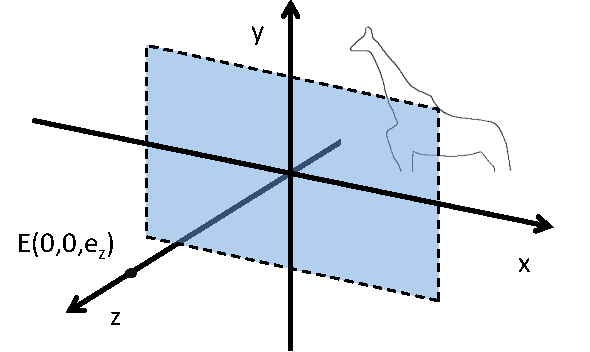
\includegraphics[width=0.7\linewidth]{images/fig17.pdf}
\caption{A coordinate system where a 3D object is projected upon a 2D plane.}
\label{fig:17}
\end{figure}

A 2D template is the image of a 3D object projected onto a 2D plane. 
Based on computer graphic theory, we build a coordinate system in \figurename~\ref{fig:17}, 
where $E(0,0,e_z)$ is the viewpoint, $O$ is the origin, $XOY$ is the imaging plane, 
and a giraffe is found in the direction of the negative $y$-axis.
If $P(x_i,y_i,z_i)$ is a point on that giraffe, 
then its projective point on the imaging plane is
\begin{equation}
x_i^{pre}=\frac{e_z x_i}{-z_i+e_z}, y_i^{pre}=\frac{e_z y_i}{-z_i+e_z}, z_i^{pre}=0.
\label{eqn:2}
\end{equation}
We use the subscript `pre' to denote the projective points of the original template before any transformations.
The subscript `post' denotes the projective points of the transformed template.

To obtain a transformed template viewed from a different angle,
we rotate the 2D template of giraffe about the $y$-axis.
If the giraffe rotates $\theta$ degree, which is equivalent to a change in viewing angle, 
then the new coordinate of $P$ is given as follows. 
\begin{eqnarray}
x_i^{rotated}&=&x_i \cos\theta+z_i \sin\theta, \nonumber\\
y_i^{rotated}&=&y_i, \nonumber\\
z_i^{rotated}&=&-x_i \sin\theta+z_i \cos\theta. 
\end{eqnarray}

Then, the projective point of the rotated $P(x_i^{rotated},y_i^{rotated},z_i^{rotated})$ on the imaging plane is as follows.
\begin{eqnarray}
x_i^{post}&=&\frac{e_z(x_i \cos\theta+z_i \sin\theta)}{x_i \sin\theta-z_i \cos\theta+e_z}, \nonumber\\
y_i^{post}&=&\frac{e_z y_i}{x_i \sin\theta-z_i \cos\theta+e_z}, \nonumber\\
z_i^{post}&=&0.
\label{eqn:4}
\end{eqnarray}

The projective points of the rotated template form the second 2D template.
From (\ref{eqn:2}) and (\ref{eqn:4}), we obtain the following.
\begin{eqnarray}
\frac{x_i^{post}}{x_i^{pre}}&=&\frac{x_i \cos\theta+z_i \sin\theta}{x_i \sin\theta-z_i \cos\theta+e_z}
\cdot\frac{-z_i+e_z}{x_i} \nonumber\\
\frac{y_i^{post}}{y_i^{pre}}&=&\frac{-z_i+e_z}{x_i \sin\theta-z_i \cos\theta+e_z} \nonumber\\
\frac{x_i^{post}}{y_i^{post}}
&=&\left(\cos\theta+\frac{z_i}{x_i}\sin\theta\right)\cdot\frac{x_i^{pre}}{y_i^{pre}}.
\label{eqn:5}
\end{eqnarray}

At present, 
we have a 2D image of the giraffe from which we cannot know the accurate parameters of the perspective projection. 
We must therefore derive another 2D image based upon the known image. 
From (\ref{eqn:5}), we can see that it is not necessary to know these parameters when we derive a new image based on an old angle of view by shifting to a new angle of view. 
In (\ref{eqn:5}), $\frac{y_i^{post}}{y_i^{pre}}$ is known,
and $\frac{z_i}{x_i}$ is determined by the original posture of the object to be detected. 
$\frac{z_i}{x_i}$ is nearly the cotangent value of one-half of the observer's horizontal visual angle. 
In human beings, this is usually implemented by a physiological mechanism occurring in the posterior parietal cortex for calculating the gazing angle and converging angle. 
Herein, we approximate this by a series of cotangent values of small angles, 
and, simultaneously, $\theta$ can also be assessed by the observer. 
If an empirical formula for assessing these values can be obtained, 
the value of $\frac{x_i^{post}}{y_i^{post}}$ can be estimated. 
In consideration for the object rotating about the $y$-axis, we have $y_i^{post}=y_i^{pre}$, 
and, finally, we can obtain $x_i^{post}$. 
This process realizes the derivation of a new 2D appearance of an object from its current 2D status without knowing the explicit perspective parameters. 
Of course, this is subject to the experiential knowledge of an observer on assessing the cotangent value of one-half of the horizontal visual angle and the variation of the visual angle.

\subsection{Variation of postures}

Another frequent factor that can change the contour of a giraffe's 2D projection is the variation of its physical posture. 
A posture rotation can be expressed by some points of a contour rotating $\theta$ degree about a line $L$, 
where $L$ is defined by a point $Q$ and a unit vector $\mathbf{u}=(u_1,u_2,u_3)$. 
In computer graphic theory, this transform is performed by a matrix $Rot(\mathbf{u},\theta)=$
\begin{equation}
\left(
\begin{array}{ccc}
 c+\bar{c}u_1^2 
& \bar{c}u_1 u_2+u_3 s 
& \bar{c}u_1 u_3-u_2 s \\
 \bar{c}u_1 u_2-u_3 s 
& c+\bar{c}u_2^2 
& \bar{c}u_2 u_3+u_1 s \\
 \bar{c}u_1 u_3+u_2 s 
& \bar{c}u_2 u_3-u_1 s 
& c+\bar{c}u_3^2
\end{array}\right),
\label{eqn:6}
\end{equation} 
where $s=\sin\theta$,$c=\cos\theta$, and $\bar{c}=1-\cos\theta$.

As an example, we suppose that a giraffe's neck has a rotational axis parallel to the $z$-axis; 
thus, $\mathbf{u} = (0,0,1)$. 
This rotation will change the coordinates of the giraffe's head and neck as follows.
\begin{equation}
(x_i^{neck},y_i^{neck},z_i^{neck},1)=(x_i,y_i,z_i,1)\cdot Rot((0,0,1),\theta).
\label{eqn:7}
\end{equation}

From equation (\ref{eqn:6}) and (\ref{eqn:7}), we get
\begin{eqnarray}
x_i^{neck}&=&x_i\cos\theta-y_i\sin\theta\nonumber\\
y_i^{neck}&=&x_i\sin\theta+y_i\cos\theta\nonumber\\
z_i^{neck}&=&z_i.
\end{eqnarray}

The projective point of the bended neck is as follows.
\begin{eqnarray}
x_i^{post}&=&\frac{e_z(x_i\cos\theta-y_i\sin\theta)}{-z_i+e_z}, \nonumber\\
y_i^{post}&=&\frac{e_z(x_i\sin\theta+y_i\cos\theta)}{-z_i+e_z}, \nonumber\\
z_i^{post}&=&0.
\label{eqn:9}
\end{eqnarray}

Comparing (\ref{eqn:9}) with the projective points of the original template in (\ref{eqn:2}),
we obtain the following.
\begin{eqnarray}
\frac{x_i^{post}}{x_i^{pre}}&=&\cos\theta-\frac{y_i}{x_i}\sin\theta \nonumber\\
\frac{y_i^{post}}{y_i^{pre}}&=&\cos\theta+\frac{x_i}{y_i}\sin\theta
\label{eqn:10}
\end{eqnarray}

In (\ref{eqn:10}), $\theta$ is assessed by the observer, 
and $\frac{y_i}{x_i}$ is obtained from the original posture of the object. 
The right-hand side of (\ref{eqn:10}) is actually the product of the tangent of one-half of the horizontal visual angle and the cotangent of one-half of the vertical visual angle. 
These are determined by the aforementioned physiological mechanism in the posterior parietal cortex, 
and these are right our visual experiences. 
Because $x_i^{pre}$ and $y_i^{pre}$ are known, $x_i^{post}$ and $y_i^{post}$ can be estimated. 
In a similar fashion, we can derive the local changes of the 2D image caused by other posture rotations. 
A complex posture rotation will be decomposed into several simple rotations about various axes.

From the proposed method based on the 2D appearance of an object, 
the knowledge of its 3D structure, and the perspective projection formulas, 
a new 2D appearance can be derived. 
This method will be used to derive a new 2D template of an object based on an existing 2D template. 
A prototype database is used to store these templates, 
which improve the generalization ability of the proposed shape-based object recognition method.

\section{Experimental Results}

\subsection{Image representation test}

Our first experiment seeks to determine whether the hypercolumn-based array is able to preserve the major contours in an original image. 
For this test, we selected the well-known contour testing dataset, MPEG-7, consisting of 1400 images. 
Similar to the method proposed in \cite{russ1995}, 
we also define the differences between the benchmark and the hypercolumn array's output as noise, 
and the signal-to-noise ratio (SNR) as $SNR[dB]=10\cdot\log_10(\frac{\sigma_{image}}{\sigma_{noise}})$.

\begin{figure}[!t]
\centering
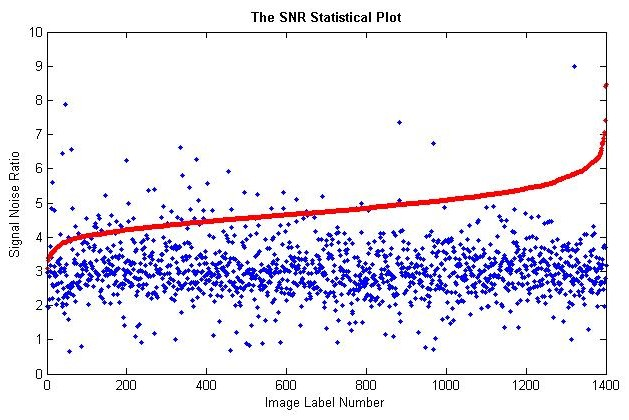
\includegraphics[width=0.95\linewidth]{images/fig18.jpg}
\caption{SNR result for the proposed method applied on the MPEG-7 dataset.}
\label{fig:18}
\end{figure}

The statistical curves shown in \figurename~\ref{fig:18}, 
where the red points are our SNR values and the blue points are the SNR values obtained from the gPb algorithm 
\cite{maire2008}, indicate that our SNR results are better than those of the gPb algorithm.
\figurename~\ref{fig:19} demonstrates three reconstruction examples,
in which column (a) includes original images from the ETHZ dataset, 
column (b) includes corresponding edge images, 
and column (c) includes re-descriptions of the edge images using routes.
\figurename~\ref{fig:20} is an example of the process of adding routes one-by-one, 
from which we observe that an image has been reduced to a small number of routes, and the route becomes the basic unit being manipulated.

\begin{figure}[!t]
\centering
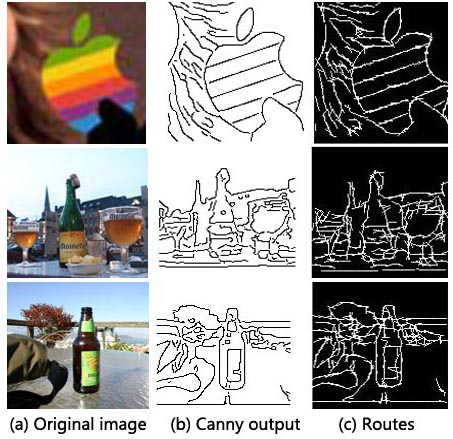
\includegraphics[width=0.9\linewidth]{images/fig19.jpg}
\caption{Representing images in the ETHZ dataset by routes.}
\label{fig:19}
\end{figure}

\begin{figure}[!t]
\centering
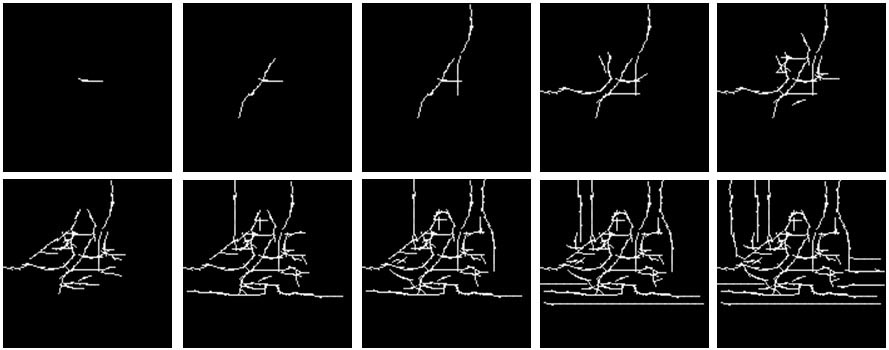
\includegraphics[width=0.95\linewidth]{images/fig20.jpg}
\caption{A sequence of routes that have been added successively.}
\label{fig:20}
\end{figure}

\subsection{Object detection test}

The most common method of evaluating object detection performance is through the use of the DR-FPPI curve, 
where DR represents the detection rate, and FPPI is the false positives per image. 
Generally, a small FPPI value can better reflect the performance of an algorithm because the DR can attain a high value provided the FPPI is loosened. 
Therefore, we prefer a smaller FPPI value such as 0.3 or 0.4. 
\tablename~\ref{tab:1} lists a comparison of DR values obtained by our method and several state-of-the-art methods 
\cite{ferrari2010,ferrari2008} for FPPI values of 0.2 and 0.4 with images obtained from the ETHZ dataset. 
\tablename~\ref{tab:1} indicates that the performance of our method is either the best or very nearly the best for all images and FPPR values considered.
 
\begin{table}[!t]
\renewcommand{\arraystretch}{1.3}
\caption{Comparison of the detection rate for FPPI 0.2/0.4}
\label{tab:1}
\centering
\scriptsize
\begin{tabular}{l|lllll}
\hline
& Apple & Bottle & Giraffe & Mug & Swan \\
\hline
Our method
& \textbf{0.80}/0.83
& 0.78/0.91
& \textbf{0.77/0.80}
& 0.75/\textbf{0.88}
& \textbf{0.75/0.81}\\
$\text{Hough only}_\text{(Pascal)}$
& 0.18/0.29
& 0.48/0.56
& 0.16/0.35
& 0.20/0.36
& 0.29/0.46\\
$\text{Full system}_\text{(Pascal)}$
& 0.74/\textbf{0.84}
& 0.69/0.82
& 0.34/0.45
& 0.66/0.79
& 0.53/0.70\\
$\text{Full system}_\text{(20\% IoU)}$
& -/-
& 0.72/0.83
& 0.47/0.59
& 0.72/0.84
& 0.63/0.75\\
$\text{Ferrari08}_\text{(Pascal)}$
& 0.38/0.60
& \textbf{0.84/0.94}
& 0.43/0.51
& 0.65/0.78
& 0.41/0.54\\
$\text{Ferrari08}_\text{(20\% IoU)}$
& 0.55/0.85
& 0.82/0.90
& 0.73/0.79
& \textbf{0.78}/0.81
& 0.47/0.64\\
\hline
\end{tabular}
\end{table}

The Weizzman dataset of horse images is another popular dataset for object detection testing. 
\figurename~\ref{fig:21} presents our testing results on this dataset. 
The three green arrowed curves represent the template segments, 
the blue curves are the successfully matched contours, and the red boxes indicate the positions of horses.

\begin{figure}[!t]
\centering
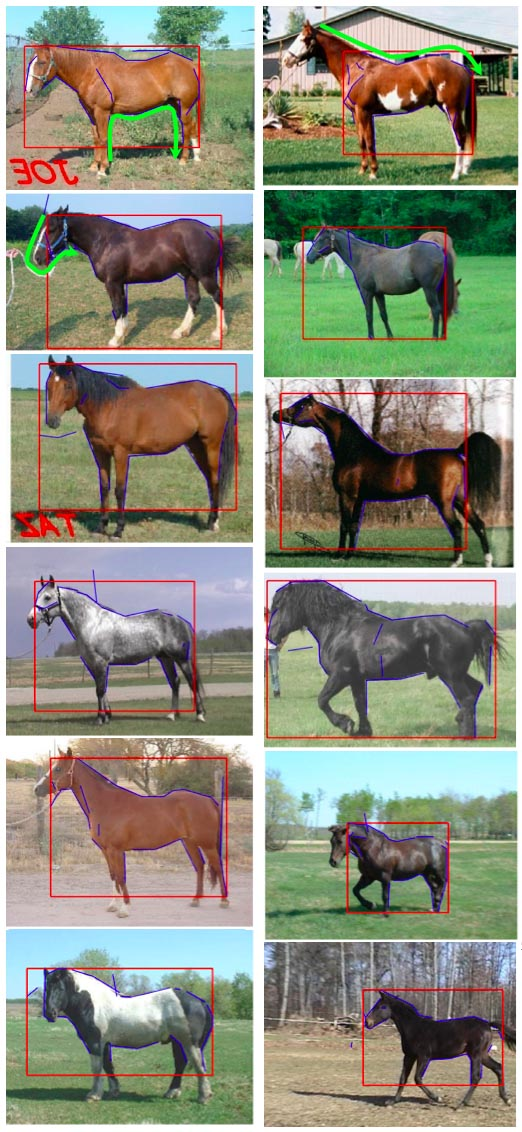
\includegraphics[width=0.95\linewidth]{images/fig21.jpg}
\caption{Detection testing for the Weizzman horse dataset.}
\label{fig:21}
\end{figure}

\subsection{Efficiency comparison}

The proposed shape-based object detection method requires no expensive training and no high-dimensional feature vectors. We therefore expect our method to exhibit a relatively high efficiency. 
To this end, we compared the time consumed for our method relative to that of a similar state-of-the-art method. 
Ma et al. \cite{ma2011} proposed a shape-based object detection method that, 
like the proposed method, utilizes contour segments as the feature of interest. 
Based again on the ETHZ dataset, we collected the time costs of the two methods.
\figurename~\ref{fig:22} shows the time comparisons for each category, 
i.e., giraffe, apple logo, swan, bottle, and mug. 
We can see that our method is much less time consuming than the other method, 
which requires exhaustive searching.

\begin{figure*}[!t]
\centering
\subfloat[Giraffes in ETHZ]{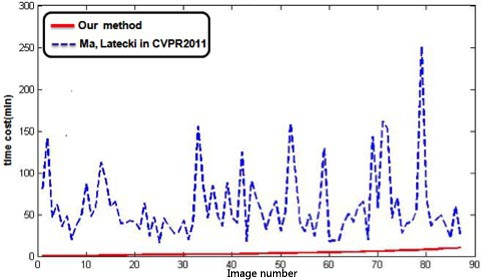
\includegraphics[width=0.33\linewidth]{images/fig22a.jpg}}\hfil%
\subfloat[Apple logos in ETHZ]{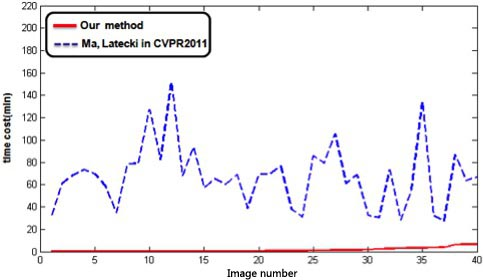
\includegraphics[width=0.33\linewidth]{images/fig22b.jpg}}\hfil%
\subfloat[Swans in ETHZ]{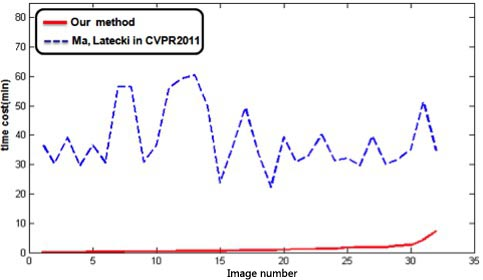
\includegraphics[width=0.33\linewidth]{images/fig22c.jpg}}\\%
\subfloat[Bottles in ETHZ]{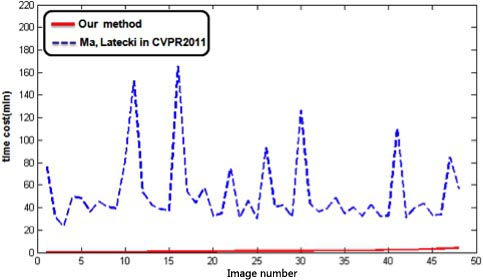
\includegraphics[width=0.33\linewidth]{images/fig22d.jpg}}\hfil%
\subfloat[Mugs in ETHZ]{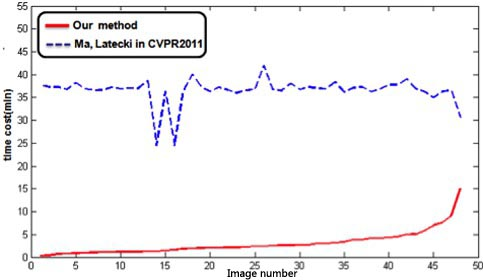
\includegraphics[width=0.33\linewidth]{images/fig22e.jpg}}%
\caption{Time-cost comparison between our method and \cite{ma2011}}
\label{fig:22}
\end{figure*}

\subsection{Active processing}

The proposed method has a pronounced potential for employing high-level knowledge downwards to actively search an image and collect specific or anticipated geometrical or topological evidence, 
a process denoted as active processing, or active image analysis. 
For example, due to some less than ideal preprocessing parameters, 
a contour segment of an object might be missed at the early phase of analysis, 
or a crucial contour might be broken into several discontinuous parts, 
or a contour misjoined with an edge from the background. 
All these errors can hide valuable evidence and prevent objects from being resolved from the background. 
However, our method has the capability of correcting these early errors at a later stage through active analysis. 
Based on a partial match between a template and some real curves, 
our method can formulate a hypothesis and anticipate what should be the next evidence and where it most likely occurs. 
Subsequently, a series of intensive operations confined to this designated and limited area are conducted, 
such as adjusting parameters, executing a new round of preprocessing, 
and facilitating the emergence of new evidence or reorganizing old evidence and searching within them. 
This type of processing, under a clear top-down instruction, is active. 
The most significant advantage of this functionality is that it enables bidirectional, data-driven, 
and concept-driven processing, and merges them together seamlessly. 
This functionality greatly improves self-adaptability.
  
\figurename~\ref{fig:23} demonstrates how active processing is achieved. 
In \figurename~\ref{fig:23}a, a suspected route is selected as the beginning of the search because it matches a part of the template well. 
This segment is re-represented by a route, i.e., a sequence of nodes. 
We define a state evaluation function for the search process, 
which is the aforementioned distance value between the current curve and the template. 
This value, as heuristic information, can be used to guide the search. 
The present distance value is 20. 
In \figurename~\ref{fig:23}b, through loosening the threshold defining neighboring nodes, 
one end node of the red route, 14, has two succeeding nodes, 15 and 19. 
A tentative, depth-first exploration can return a value of the state evaluation function. 
The movement towards 15 brings a value of 17.98, and that towards 19 brings a value of 15.54, 
making the second candidate the better choice, which leads us to \figurename~\ref{fig:23}c. 
From \figurename~\ref{fig:23}d~to~\ref{fig:23}e the remaining nodes can be evaluated in the same manner, 
where only the node with the smallest heuristic value can be extended. 
In particular, \figurename~\ref{fig:23}e indicates that a region-limited preprocessing is executed again under a new canny-detector parameter because the active processing attempts to find a permanently lost edge that bridges the gap between two routes. 
Finally, as shown in \figurename~\ref{fig:23}f, an almost perfect contour of a bottle is fully detected.

\begin{figure}[!t]
\centering
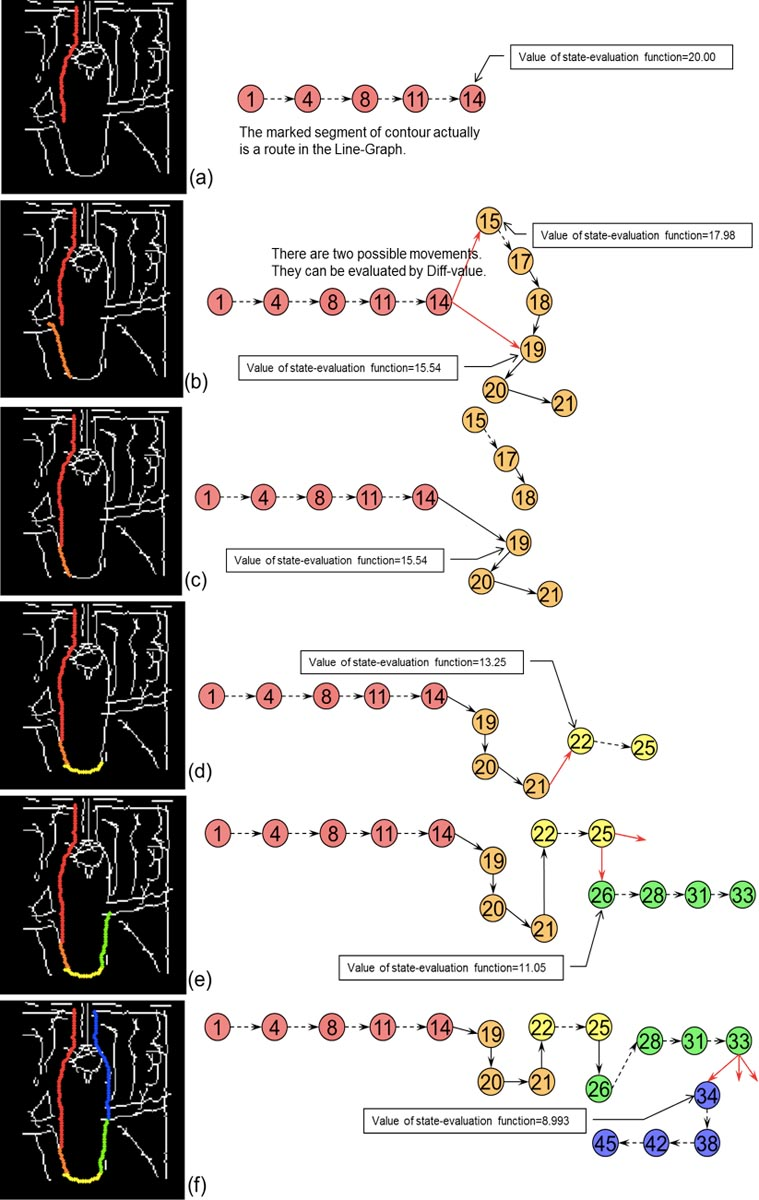
\includegraphics[width=0.98\linewidth]{images/fig23.jpg}
\caption{An illustration of active-processing.}
\label{fig:23}
\end{figure}

In principle, active processing can be realized under any kind of image representation. 
However, in practice, an overly fine representation is harmful for efficiency, 
and an overly abstract representation is harmful for flexibility. 
The Line-graph and Route-graph mechanism is able to not only integrate discrete pixels to a compound degree, 
but also preserve sufficient details for intensive analysis. 
This mechanism not only facilitates searching, 
but also significantly eases the burden associated with the searching process.

\section{Conclusion}

\figurename~\ref{fig:24} briefly summaries the overall architecture of the proposed system.

\begin{figure}[!t]
\centering
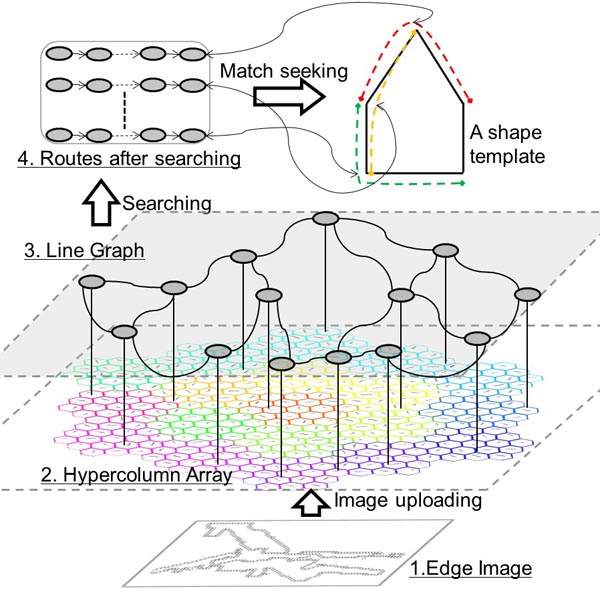
\includegraphics[width=0.95\linewidth]{images/fig24.jpg}
\caption{The overall architecture of the proposed system.}
\label{fig:24}
\end{figure}

The system has four representation levels: 
(1) an edge image; (2) a hypercolumn-array representing the contour information of the edge image; 
(3) a graph of neighboring short line segments; 
and (4) the salient routes of the graph that are candidates for shape matching. 
The most significant aspect of this process is that the route of a graph provides the proper granularity for the operations of shape-construction and shape-destruction, i.e., the route is sufficiently flexible and concise to be manipulated for the purpose of contour combination.

Therefore, the present work provides the following four conclusions.

(a) Perception always is real-time processing, so its efficiency is crucial for an algorithm's rationality evaluation. In this paper, we achieve the same performance using a relatively simple method, but our method is much more time-saving.

(b) A biological visual system, especially that of a mammal, has been evolved by nature to be a highly optimized system. Feature-integration theory has been deeply studied in cognitive psychology. Physiological inspirations are indispensable for designing a practical vision system.

(c) Task-specific methods, for their diversities, are weak to mature vision theory. A necessary symbol for this theory is it has a unique architecture, whether in representation or in processing. For this sake, choosing geometrical structure and topological relation to represent and choosing shape match to achieve recognition are perhaps on the right track.

(d) The training set and appearance-based machine learning strategy for object detection under a natural environment can never exhaust all possible negative cases. Therefore, this strategy is really too expensive for its limited gain in generalization. The strategy of evidence accumulation and inference can avoid these costs.


%\appendices
%\section{Proof of the First Zonklar Equation}
%Appendix one text goes here.

\section*{Acknowledgment}

This work was supported by the 973 Program (Project No. 2010CB327900), NSFC project (Project Nos. 61375122 and 30990260). We also thank the anonymous referees for their helpful comments.


% Can use something like this to put references on a page
% by themselves when using endfloat and the captionsoff option.
\ifCLASSOPTIONcaptionsoff
  \newpage
\fi



% trigger a \newpage just before the given reference
% number - used to balance the columns on the last page
% adjust value as needed - may need to be readjusted if
% the document is modified later
%\IEEEtriggeratref{8}
% The "triggered" command can be changed if desired:
%\IEEEtriggercmd{\enlargethispage{-5in}}

% references section

% can use a bibliography generated by BibTeX as a .bbl file
% BibTeX documentation can be easily obtained at:
% http://www.ctan.org/tex-archive/biblio/bibtex/contrib/doc/
% The IEEEtran BibTeX style support page is at:
% http://www.michaelshell.org/tex/ieeetran/bibtex/
\bibliographystyle{IEEEtran}
% argument is your BibTeX string definitions and bibliography database(s)
\bibliography{ref}
%
% <OR> manually copy in the resultant .bbl file
% set second argument of \begin to the number of references
% (used to reserve space for the reference number labels box)
%\begin{thebibliography}{1}
%
%\bibitem{IEEEhowto:kopka}
%H.~Kopka and P.~W. Daly, \emph{A Guide to \LaTeX}, 3rd~ed.\hskip 1em plus
%  0.5em minus 0.4em\relax Harlow, England: Addison-Wesley, 1999.
%
%\end{thebibliography}

% biography section


%\vfill

% that's all folks
\end{document}


